\chapter{Usage of Annotations -- Fuzzy ILP Document Classification} \label{sec:ch80_fuzzy_ilp_chapter}

\graphicspath{{../img/ch80/}}




%%%%%%%%%%%%%%%%%%%%%%%%%%%%%%%%%%%%%%%%%%%%%%%%%%%%%%%%%%%%%%%%%%%%%%%%%%%%%%%%%%%%%%%%%%%%%%%%%%
%\subsection{Linguistic Analysis}
%%%%%%%%%%%%%%%%%%%%%%%%%%%%%%%%%%%%%%%%%%%%%%%%%%%%%%%%%%%%%%%%%%%%%%%%%%%%%%%%%%%%%%%%%%%%%%%%%%
%
%See \ref{sec:ch30_ling_tools}

%In this section we will briefly describe the linguistic tools that
%we have used to produce linguistic annotations of texts. 
%These tools are being developed in the Institute of Formal
%and Applied Linguistics in Prague, Czech Republic. They
%are publicly available -- they have been published on a CDROM
%under the title PDT 2.0 (\citep{biblio:PDT20_CD} -- the first five tools) and in
%(\citep{biblio:KlTransformationBasedTectogrammatical2006} -- Tectogrammatical analysis). These tools are used as a
%processing chain. At the end of the chain they produce
%tectogrammatical dependency trees \citep{biblio:MiBeAnnotationtectogrammatical2006} built up from the text.
%
%
%\begin{description}
 %
	%\item[Tool 1.] Segmentation and tokenization consists of dividing the input text into words and punctuation (tokenization) and dividing a sequence of tokens into sentences (segmentation).
%
	%\item[Tool 2.] Morphological analysis assigns all possible lemmas
%and morphological tags to particular word forms (word
%occurrences) in the text.
%
	%\item[Tool 3.] Morphological tagging consists in selecting a single
%pair lemma-tag from all possible alternatives assigned
%by the morphological analyzer.
%
	%\item[Tool 4.] Collins' parser -- Czech adaptation. 
%Unlike the usual approaches to the description of
%English syntax, the Czech syntactic descriptions are
%dependency-based, which means that every edge of
%a syntactic tree captures the relation of dependency
%between a governor and its dependent node. Collins'
%parser gives the most probable parse of a given input
%sentence.
%
	%\item[Tool 5.] Analytical function assignment assigns a description
%(analytical function, in linguistic sense) to every edge
%in the syntactic (dependency) tree.
%
	%\item[Tool 6.] Tectogrammatical analysis produces linguistic annotation
%at the tectogrammatical level, sometimes called
%``layer of deep syntax''. An example of a tectogrammatical tree can be seen in
%Figure~\ref{img:ch80_tree}. Annotation of a sentence at this layer
%is closer to the meaning of the sentence than its syntactic
%annotation; thus, information captured at the tectogrammatical
%layer is crucial for machine understanding
%of natural language \citep{biblio:KlTransformationBasedTectogrammatical2006}.
%\end{description}


%%%%%%%%%%%%%%%%%%%%%%%%%%%%%%%%%%%%%%%%%%%%%%%%%%%%%%%%%%%%%%%%%%%%%%%%%%%%%%%%%%%%%%%%%%%%%%%%%
%\subsection{Web Information Extraction}
%%%%%%%%%%%%%%%%%%%%%%%%%%%%%%%%%%%%%%%%%%%%%%%%%%%%%%%%%%%%%%%%%%%%%%%%%%%%%%%%%%%%%%%%%%%%%%%%%

%After the content of a web resource is analyzed by the above-mentioned linguistic tools, the output linguistic data is obtained in the form of tectogrammatical trees. To achieve our objectives we have to extract information from this representation. 
%Here we refer to our previous work %\citep{biblio:DeVoComputingaggregations2008,biblio:DeVoLinguisticextraction2008,biblio:DeEcExperimentswith2008}.
%\citep{biblio:DeVoComputingaggregations2008,biblio:DeEcExperimentswith2008}.
 %A long path of tools, starting with web crawling and resulting in the extracted structured information, has been developed in our previous works. 
%In this paper we will concentrate on the usage of such extracted information to be able to classify content. 
















%There are two objectives to do. Fist is the information extraction, a long path starting with web crawling and resulting with the extracted structured information. Second is the seriousness classification, which utilizes the extracted information. We have made much work on the first (see e.g. %\citep{biblio:DeVoLinguisticextraction2008,biblio:DeVoComputingaggregations2008, biblio:DeEcExperimentswith2008}), in this paper we will concentrate on the second.
%\citep{biblio:DeEcExperimentswith2008}), in this paper we will concentrate on the second.




%\begin{table}
%\centering
%\begin{tabular}{|r||c|c|c|}
%\hline
%attribute name & distinct values & missing values & monotonic\\
%\hline
%\hline
%size (of file) & 49 & 0 & yes\\
%\hline
%type (of accident) & 3 & 0 & no\\
%\hline
%damage & 18 & 30 & yes\\
%\hline
%dur\_minutes & 30 & 17 & yes\\
%\hline
%fatalities & 4 & 0 & yes\\
%\hline
%injuries & 5 & 0 & yes\\
%\hline
%cars & 5 & 0 & yes\\
%\hline
%amateur\_units & 7 & 1 & yes\\
%\hline
%profesional\_units & 6 & 1 & yes\\
%\hline
%pipes & 7 & 8 & yes\\
%\hline
%lather & 3 & 2 & yes\\
%\hline
%aqualung & 3 & 3 & yes\\
%\hline
%fan & 3 & 2 & yes\\
%\hline
%ranking & 14 & 0 & yes\\
%\hline
%\end{tabular}
%
%\caption{Accident attributes.}
%\label{img:attributes_description}
%\end{table}
%
%
%%%%%%%%%%%%%%%%%%%%%%%%%%%%%%%%%%%%%%%%%%%%%%%%%%%%%%%%%%%%%%%%%%%%%%%%%%%%%%%%%%%%%%%%%%%%%%%%%%
%\subsection{Features of accidents} \label{sec:features}
%%%%%%%%%%%%%%%%%%%%%%%%%%%%%%%%%%%%%%%%%%%%%%%%%%%%%%%%%%%%%%%%%%%%%%%%%%%%%%%%%%%%%%%%%%%%%%%%%%
%
%
%Table~\ref{img:attributes_description} summarizes all features (or attributes) that we have obtained from accident reports. Except for the attribute \verb+type+ (type of an accident -- \verb+fire+, \verb+car_accident+ and \verb+other+), all the attributes are numerical and therefore \emph{monotonizable} (see the next sections). There are cases in which the value of an attribute is unknown. We have decided to make evidence of this and keep the values \verb+unknown+ in the knowledge base. A brief explanation of each attribute follows.
%\begin{itemize}
	%\item \verb+size+ is length of text of a particular report.
	%\item \verb+damage+ is an amount (in CZK -- Czech Crowns) of summarized damage arisen during a reported accident.
	%\item \verb+dur_minutes+ is time taken to handle an accident.
	%\item \verb+fatalities+ and \verb+injuries+ are numbers of deaths and wound people sustained in an accident.
	%\item \verb+cars+ is the number of vehicles damaged during an accident (mostly during car accidents).
	%\item \verb+professional_units+ and \verb+amateur_units+ are numbers of fireman and volunteer units sent for a particular accident.
	%\item \verb+pipes+ is a number of used fire hoses.
	%\item \verb+lather+, \verb+aqualung+ and \verb+fan+ (ventilator) indicates whether these devices were used.
%\end{itemize}
%
%A majority of accidents are of the type \verb+fire+ (52\%)
%and \verb+car_accident+ (30\%),
%the rest (type \verb+other+, 18\%)
%deals with ecological disasters, chemical accidents, etc.
%
%%%%%%%%%%%%%%%%%%%%%%%%%%%%%%%%%%%%%%%%%%%%%%%%%%%%%%%%%%%%%%%%%%%%%%%%%%%%%%%%%%%%%%%%%%%%%%%%%%
%\subsection{Seriousness ranking} \label{sec:seriousness}
%%%%%%%%%%%%%%%%%%%%%%%%%%%%%%%%%%%%%%%%%%%%%%%%%%%%%%%%%%%%%%%%%%%%%%%%%%%%%%%%%%%%%%%%%%%%%%%%%%
%
%%\vspace{0.2cm}
%%\noindent \textbf{Seriousness ranking}
%
%\begin{figure}
%\centerline{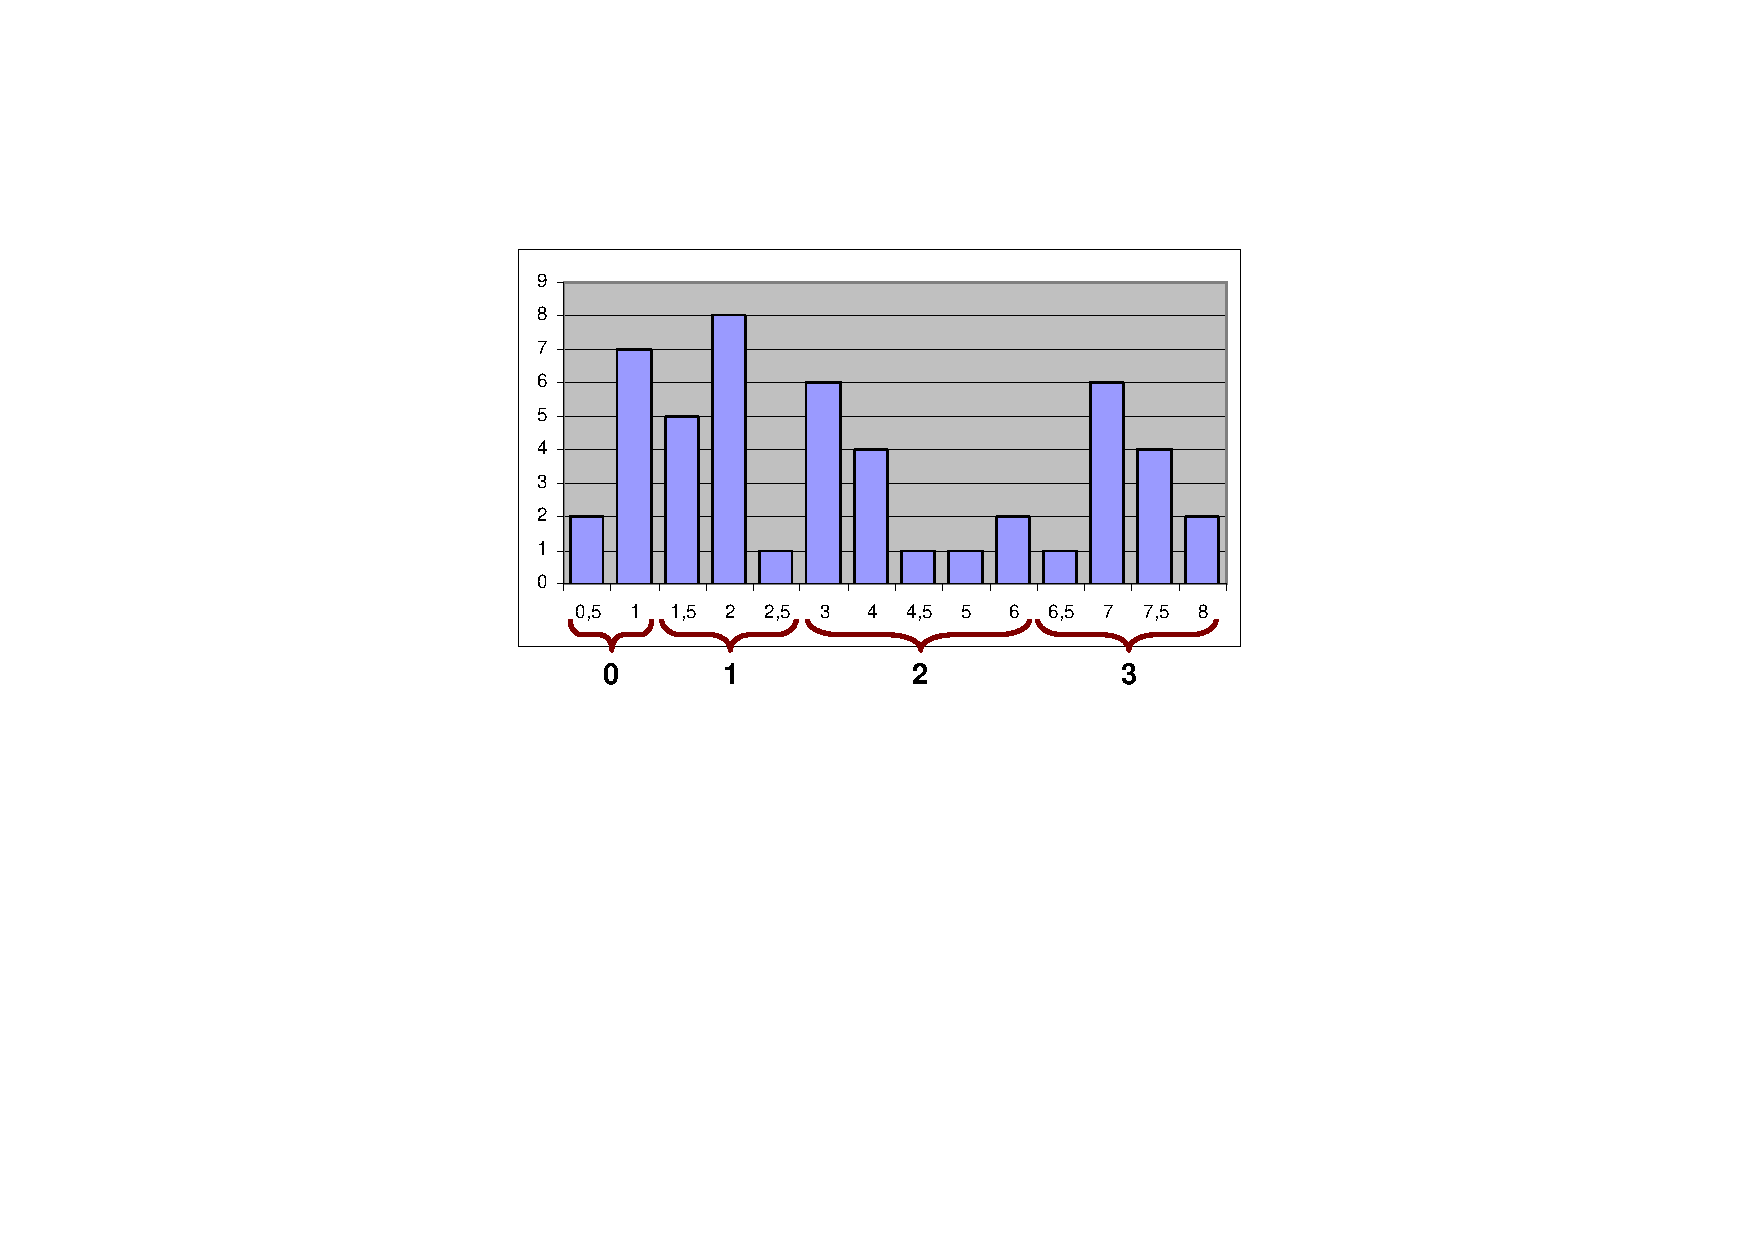
\includegraphics[angle=-90, width=0.6\hsize]{ranking_histogram}}
%\caption{Frequencies of the seriousness ranking.}
%\label{img:ranking_histogram}
%\end{figure}
%
%Values of the overall seriousness ranking attribute were stated from ``a general impression'' made by the texts with respect to particular attributes. %(Figure~\ref{img:attributes_description}). 
%The values have evolved to 14 distinct values in the range from 0.5 to 8. 
%A histogram with frequencies of all these values is in Figure~\ref{img:ranking_histogram}.
%We have divided the values into four approximately equipotent groups 
%(see in Figure~\ref{img:ranking_histogram}) 
%and these groups determine the target class attribute of the classification task. 
%%and logic rules were learned for each group separately\footnote{We do not have a binary rule, which would return an exact value of the rating, but we have one ``true/false'' rule for each of the four categories.}.
%
%






%%%%%%%%%%%%%%%%%%%%%%%%%%%%%%%%%%%%%%%%%%%%%%%%%%%%%%%%%%%%%%%%%%%%%%%%%%%%%%%%%%%%%%%%%%%%%%%%%
%\section{Evaluation} \label{sec:ch80_eval}
%%%%%%%%%%%%%%%%%%%%%%%%%%%%%%%%%%%%%%%%%%%%%%%%%%%%%%%%%%%%%%%%%%%%%%%%%%%%%%%%%%%%%%%%%%%%%%%%%




%%%%%%%%%%%%%%%%%%%%%%%%%%%%%%%%%%%%%%%%%%%%%%%%%%%%%%%%%%%%%%%%%%%%%%%%%%%%%%%%%%%%%%%%%%%%%%%%%
\section{Conclusion} \label{sec:conclusion}
%%%%%%%%%%%%%%%%%%%%%%%%%%%%%%%%%%%%%%%%%%%%%%%%%%%%%%%%%%%%%%%%%%%%%%%%%%%%%%%%%%%%%%%%%%%%%%%%%
In this chapter we have presented a fuzzy system, which provides a fuzzy classification of textual reports. Our approach is based on usage of third party linguistic analyzers, our previous work on information extraction, and fuzzy inductive logic programming.

The main contributions are formal models, prototype implementation of the presented methods and an evaluation experiment. Our data and our implementation are publicly available on the Web. The first experiment evaluated performance of the presented methods and compared them with other machine learning procedures used in data mining on our data. The Fuzzy ILP classifier proved better results than a majority of the methods. The results are statistically significant in many cases. 
We see the advantage of the Fuzzy ILP classifier in the fact that monotonization leads to the extension of the learning domain and it utilizes the fact that the domain is or can be monotonically ordered.

In the second experiment, we evaluated all the methods on other datasets with more training instances and we also experimentally measured the time complexity of the methods. This experiment has shown that the fuzzy method is suitable mainly in situations with a small amount of training instances and in cases when the target attribute mostly respects the natural order of the remaining attributes. But this did not hold true for any of the later-used datasets. When comparing the fuzzy approach with the crisp one, the fuzzy approach always performed better in terms of correctness of the classification, but it was many times slower than all the methods in terms of time complexity.
